\hypertarget{ImageProcess_8cpp}{}\section{src/\+Image\+Process.cpp File Reference}
\label{ImageProcess_8cpp}\index{src/\+Image\+Process.\+cpp@{src/\+Image\+Process.\+cpp}}


This node takes and analyze the range data. Subsequently, pass the the decision made based on the data to the turtle\+Ctrl node which manipulates the turtlebot.  


{\ttfamily \#include $<$ros/ros.\+h$>$}\\*
{\ttfamily \#include $<$opencv2/core/core.\+hpp$>$}\\*
{\ttfamily \#include $<$opencv2/opencv.\+hpp$>$}\\*
{\ttfamily \#include \char`\"{}opencv2/highgui/highgui.\+hpp\char`\"{}}\\*
{\ttfamily \#include \char`\"{}opencv2/imgproc/imgproc.\+hpp\char`\"{}}\\*
{\ttfamily \#include \char`\"{}Image\+Process.\+hpp\char`\"{}}\\*
Include dependency graph for Image\+Process.\+cpp\+:\nopagebreak
\begin{figure}[H]
\begin{center}
\leavevmode
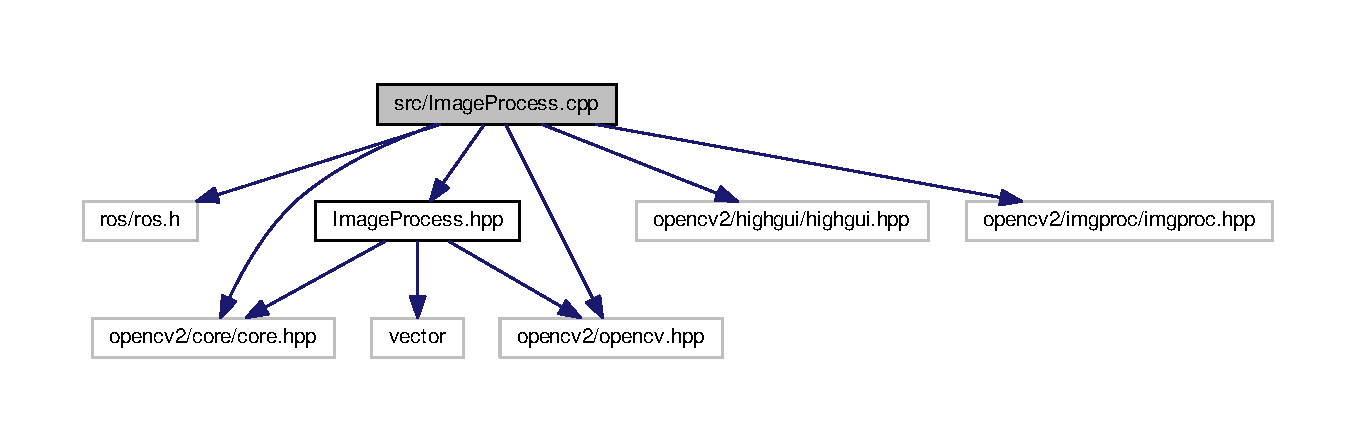
\includegraphics[width=350pt]{ImageProcess_8cpp__incl}
\end{center}
\end{figure}


\subsection{Detailed Description}
This node takes and analyze the range data. Subsequently, pass the the decision made based on the data to the turtle\+Ctrl node which manipulates the turtlebot. 

\begin{DoxyAuthor}{Author}
Yuyu Hsueh  2017, Yuyu Hsueh 
\end{DoxyAuthor}
